%%%%%%%%%%%%%%%%%%%%%%%%%%%%%%%%%%%%%%%%%%%%%%%%%%%%%%%%%%%%%%%%%%%%%%%%%%%%%%%%%%
\begin{frame}[fragile]\frametitle{}
\begin{center}
{\Large References}
\end{center}
\end{frame}


%%%%%%%%%%%%%%%%%%%%%%%%%%%%%%%%%%%%%%%%%%%%%%%%%%%%%%%%%%%
\begin{frame}[fragile]\frametitle{Sources Referred}

Many publicly available sources have been used in the preparation of this content. Some of the salient ones are listed below:

	\begin{itemize}
	\item An Ultimate Guide to 15 Most Popular Types of Yoga - Naveen Sharma
	\item The Yoga Sutras of Patanjali - Prof. Edwin Bryant
	\item योग सूत्र का परिचय | Yoga Sutras of Patanjali | Yoga Sutras For QCI, UGC NET, Yoga All Exams - YouTube
	\item योग का अर्थ एवं परिभाषा | योग का संपूर्ण परिचय | Meaning Of Yoga For QCI, UGC NET, Yoga All Exams - YouTube
	\item Patanjali Yoga Sutra Dr Mrudula Chaudhari
	\item Patanjali Yoga Sutras | Explanation by Anandmurti Gurumaa Gurumaa Ashram Verified
	\item Yoga Sutra, Bhagavad Gita; a conversation with Edwin Bryant Part 1 - YouTube
	\end{itemize}

\end{frame}


%%%%%%%%%%%%%%%%%%%%%%%%%%%%%%%%%%%%%%%%%%%%%%%%%%%%%%%%%%%
\begin{frame}[fragile]\frametitle{}

\begin{center}
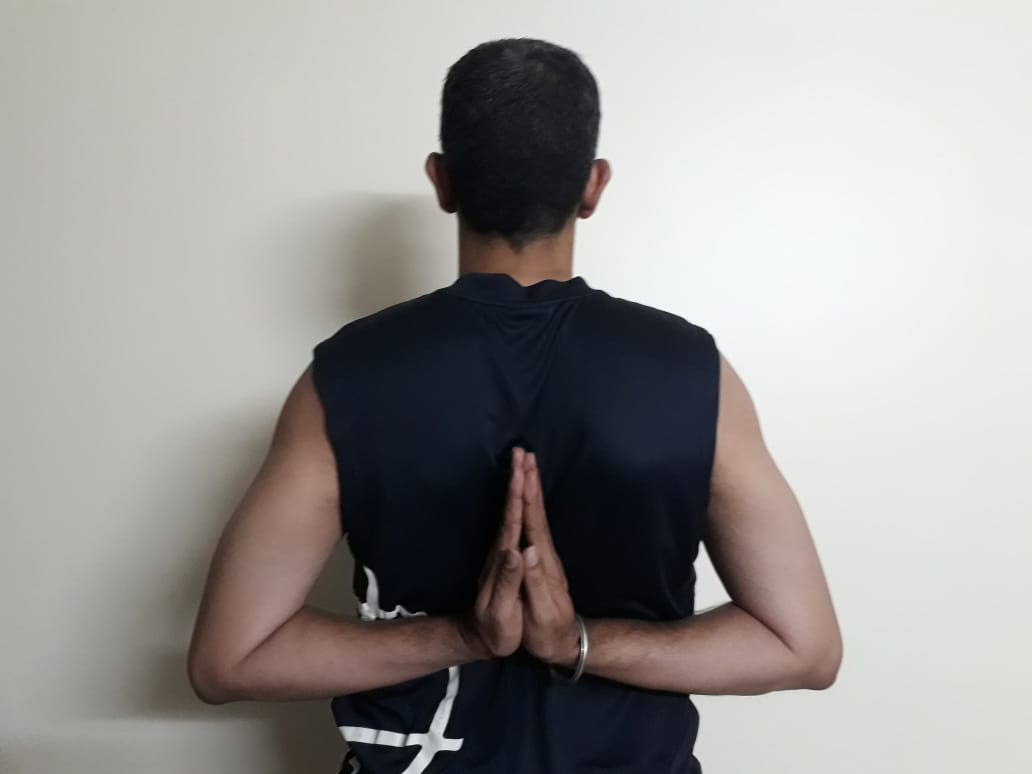
\includegraphics[width=0.8\linewidth,keepaspectratio]{my_yog_back}

Thanks धन्यवाद
\end{center}

\end{frame}